\documentclass[12pt,letterpaper, onecolumn]{exam}
\usepackage{amsmath}
\usepackage{amssymb}
\usepackage{listings}
\usepackage[lmargin=71pt, tmargin=1.2in]{geometry}  %For centering solution box
\usepackage{graphicx}
\lhead{IF5152 Computer Vision\\}
\rhead{Assignment 2 (18221101)\\}

% \chead{\hline} % Un-comment to draw line below header
\thispagestyle{empty}   %For removing header/footer from page 1

\begin{document}

\begingroup  
    \centering
    \LARGE IF5152  Computer Vision\\
    \LARGE Assignment 2 Writeup\\[0.5em]
    \large November 5, 2024 \\[0.5em]
    \large Ilmagita Nariswari\par
    \large 18221101\par
    \large Semester Ganjil 2024/2025\par
\endgroup
\rule{\textwidth}{0.4pt}
\pointsdroppedatright   %Self-explanatory
\printanswers
\renewcommand{\solutiontitle}{\noindent\textbf{Ans:}\enspace}   %Replace "Ans:" with starting keyword in solution box

\begin{questions}

    \question \textbf{Q1.2 Correspondences} \\
    
    Let \(\mathbf{x_1}\) be a set of points in an image and \(\mathbf{x_1}\) be the set of corresponding points in an image taken by another camera. Suppose there exists a homography \(\mathbf{H}\) such that:
    
    \begin{center}
        \(\mathbf{x_1^i} \equiv \mathbf{H} \mathbf{x_2^i} \quad (i \in \{ 1 \dots N \})\)
    \end{center}
    
    where \(\mathbf{x_1^i} = \begin{bmatrix} x_1^i & y_1^i & 1 \end{bmatrix}^T\) are in homogeneous coordinates, \(\mathbf{x_1^i} \in \mathbf{x_1}\), and \(\mathbf{H}\) is a \(3 \times 3\) matrix. For each point pair, this relation can be rewritten as
    \begin{center}
        \(\mathbf{A_ih = 0}\)
    \end{center}
    where \(\mathbf{h}\) is a column vector reshaped from \(\mathbf{H}\), and \(\mathbf{A_i}\) is a matrix with elements derived from points \(\mathbf{x_1^i}\) and \(\mathbf{x_2^i}\). This can help calculate \(\mathbf{H}\) from the given point correspondences.

    \begin{enumerate}
        \item How many degrees of freedom does \(\mathbf{h}\) have?
        \item How many point pairs are required to solve \(\mathbf{h}\)? 
        \item Derive \(\mathbf{A_i}\).
        \item When solving \(\mathbf{Ah = 0}\), in essence you're trying to find the \(\mathbf{h}\) that exists in the null space of \(\mathbf{A}\). What that means is that there would be som non-trivial solution for \(\mathbf{h}\) such that product \(\mathbf{Ah}\) turns out to be 0. What will be a trivial solution for \(\mathbf{h}\)? Is the matrix \(\mathbf{A}\) full rank? Why/why not? What impact will it have on the eigen values? What impact will it have on the eigen vectors?
    \end{enumerate}
    
    \begin{solution}
        \begin{enumerate}
            \item There are 8 degrees of freedom for a homography.
            A \(\mathbf{3x3}\) matrix should have 9 degrees of freedom, but it has 8 degrees of freedom as it is estimated up to scale. Mathematically, this can be seen as 
            \[
                \begin{bmatrix} h_{11} & h_{12} & h_{13} \\ h_{21} & h_{22} & h_{23} \\ h_{31} & h_{32} & h_{33} \\ \end{bmatrix}
                \begin{bmatrix} x \\ y \\ 1 \end{bmatrix}
            \]
            \item Each point-to-point correspondence accounts for two constraints. Hence, 8 degrees of freedom account for 4 pair points at a minimum to solve for \(\mathbf{h}\).
            \item The equation
            \[
                \mathbf{x_1^i} \equiv \mathbf{H} \mathbf{x_2^i} 
            \]
            where \(\mathbf{H}\) is a matrix can be written to
            \\
            \[
                \begin{bmatrix} x_1^i \\ y_1^i \\ 1 \end{bmatrix} = \begin{bmatrix} h_{11} & h_{12} & h_{13} \\ h_{21} & h_{22} & h_{23} \\ h_{31} & h_{32} & h_{33} \\ \end{bmatrix} \begin{bmatrix} x_2^i \\ y_2^i \\ 1 \end{bmatrix} 
            \]
            \\
            which can be expanded into
            \[
                x_1^i = h_{11}x_2^i + h_{12}y_2^i + h_{13}
            \]
            \[
                y_1^i = h_{21}x_2^i + h_{22}y_2^i + h_{23}
            \]
            \[
                1 = h_{31}x_2^i + h_{32}y_2^i + h_{33}
            \]
            and further can be rearranged as
            \[
                x_1^i(h_{31}x_2^i + h_{32}y_2^i + h_{33}) = h_{11}x_2^i + h_{12}y_2^i + h_{13}
            \]
            \[
                y_1^i(h_{31}x_2^i + h_{32}y_2^i + h_{33}) = h_{21}x_2^i + h_{22}y_2^i + h_{23}
            \]
            We want the right side to equal 0, so
            \[
                - x_1^ih_{31}x_2^i - x_1^ih_{32}y_2^i - x_1^ih_{33} + h_{11}x_2^i + h_{12}y_2^i + h_{13} = 0
            \]
            \[
                - y_1^ih_{31}x_2^i - y_1^ih_{32}y_2^i - y_1^ih_{33} + h_{21}x_2^i + h_{22}y_2^i + h_{23} = 0
            \]
            Rearrange the above equation into a matrix yields
            \[
                \begin{bmatrix}
                    x_2^i & y_2^i & 1 & 0 & 0 & 0 & -x_1^i x_2^i & -x_1^iy_2^i & -x_1^i \\
                    0 & 0 & 0 & x_2^i & y_2^i & 1 & -x_2^iy_1^i & -y_1^iy_2^i & -y_1^i
                \end{bmatrix}
                \begin{bmatrix}
                    h_{11} \\
                    h_{12} \\
                    h_{13} \\
                    h_{21} \\
                    h_{22} \\
                    h_{23} \\
                    h_{31} \\
                    h_{32} \\
                    h_{33} \\
                \end{bmatrix}
                = 0
            \]
            Hence, the above equation can be written in the form of
            \[
                \mathbf{A_ih = 0}
            \]
            \item The point of origin (0,0) would always be (0,0) even after transformation, so the trivial solution would be an \(\mathbf(9 \times 1)\) matrix \(\mathbf h\). Matrix A cannot be full rank because it must have a zero eigen value. The least singular value will be 0.
        \end{enumerate}
    \end{solution}

    \pagebreak

    \question \textbf{Q2.1.3 Matching Methods} \\
    The BRIEF descriptor belongs to a category called binary descriptors. In such descriptors the image region corresponding to the detected feature point is represented as a binary string of 1s and 0s. A commonly used metric used for such descriptors is called the Hamming distance. Please search online to learn about Hamming distance and Nearest Neighbor, and describe how they can be used to match interest points with BRIEF descriptors. What benefits does the Hamming distance have over a more conventional Euclidean distance measure in our setting?

    \begin{solution}
        Binary feature descriptor is a feature vector that only contains 1 and 0. BRIEF first smooths an image patch using a Gaussian kernel and creates a binary strings out of the patch by comparing pairs of pixel intensities in an image patch. Meanwhile, Hamming distance is the number of bit positions in which the two bits are different. It differens than Euclidean distance, because Euclidean takes the shortest distance between two vectors by taking the square root of the sum of squares of differences between corresponding points. \\~\\
        Mathematically, when given a pair of points \(a = (_1, \dots, a_n)\) and \(b = (b_1, \dots, b_n)\), the distance of Euclidean is noted as
        \[
            d_{Euclidean} = \sqrt{(a_1 - b_1)^2 + \dots + (a_n - b_n)^2}
        \]
        while the distance of Hamming can be computed using the XOR operation between two points.\\~\\
        It is precisely the XOR operation that is much faster than taking the square root of the sum of squares of differences that makes Hamming distance have a greater benefit than the Euclidean distance. It also works directly on the binary data and doesn't need any type conversion.
        \\~\\
        \textbf{References}
        \begin{enumerate}
            \item https://medium.com/@deepanshut041/introduction-to-brief-binary-robust-independent-elementary-features-436f4a31a0e6
            \item https://www.tutorialspoint.com/what-is-hamming-distance
            \item https://www.gaussianwaves.com/2020/09/euclidean-and-hamming-\\distances/
            \item L. Yan, H. Lu, C. Wang, Z. Ye, H. Chen, and H. Ling, "Deep linear discriminant analysis hashing for image retrieval," Multimedia Tools and Applications, vol. 78, 2019, doi: 10.1007/s11042-018-6855-y 
            \item M. Calonder, V. Lepetit, C. Strecha, and P. Fua, "BRIEF: Binary Robust Independent Elementary Features," in Proceedings of the 11th European Conference on Computer Vision (ECCV), 2010.
        \end{enumerate}
    \end{solution}

    \pagebreak

    \question \textbf{Q2.1.4 Feature Matching}\\
    Please implement a function:

    \begin{center}
    \texttt{matches, lovs1, locs2 = matchPics(I1, I2)}
    \end{center}
    
    where \texttt{I1} and \texttt{I2} are the images you want to match. \texttt{matches} is a $p \times 2$ matrix where the first column is indices into features in \texttt{I1}, and similarily the second column contains indices related to \texttt{I2}. Use the provided helper function \texttt{corner\_detection} to compute the features, then build descriptors using the provided helper function \texttt{computeBrief}, and finally compare them using the provided helper function \texttt{briefMatch}.\\ \\
    Use the provided helper function \texttt{plotMatches} to visualize your matched points and include the result image in your write-up.\\ \\
    The number of matches between the two images varies based on the parameter \texttt{sigma} used in \texttt{corner\_detection}, and also on the value \texttt{ratio} in \texttt{briefMatch}. You should vary these to get the best results.

    \begin{solution}
        Results after varying ratio and sigma:
        \begin{center}
            Table X Variations of ratio in \texttt{briefMatch} and sigma in \texttt{corner\_detection}
        \end{center}
        \begin{center}
            \begin{tabular}{|c|c|c|}
                \hline
                \textbf{Ratio} & \textbf{Sigma} & \textbf{Matches} \\
                \hline
                0.4 & 0.1 & 0 \\
                \hline
                0.4 & 0.3 & 0 \\
                \hline
                0.4 & 0.5 & 0 \\
                \hline
                0.4 & 0.7 & 0 \\
                \hline
                0.4 & 0.9 & 0 \\
                \hline
                0.5 & 0.1 & 4 \\
                \hline
                0.5 & 0.3 & 4 \\
                \hline
                0.5 & 0.5 & 4 \\
                \hline
                0.5 & 0.7 & 4 \\
                \hline
                0.5 & 0.9 & 4 \\
                \hline
                0.55 & 0.1 & 5 \\
                \hline
                0.55 & 0.3 & 5 \\
                \hline
                0.55 & 0.5 & 5 \\
                \hline
                0.55 & 0.7 & 5 \\
                \hline
                0.55 & 0.9 & 5 \\
                \hline
            \end{tabular}
            \quad
            \begin{tabular}{|c|c|c|}
                \hline
                \textbf{Ratio} & \textbf{Sigma} & \textbf{Matches} \\
                \hline
                0.6 & 0.1 & 7 \\
                \hline
                0.6 & 0.3 & 7 \\
                \hline
                0.6 & 0.5 & 7 \\
                \hline
                0.6 & 0.7 & 7 \\
                \hline
                0.6 & 0.9 & 7 \\
                \hline
                0.65 & 0.1 & 16 \\
                \hline
                0.65 & 0.3 & 16 \\
                \hline
                0.65 & 0.5 & 16 \\
                \hline
                0.65 & 0.7 & 16 \\
                \hline
                0.65 & 0.9 & 16 \\
                \hline
                0.7 & 0.1 & 27 \\
                \hline
                0.7 & 0.3 & 27 \\
                \hline
                0.7 & 0.5 & 27 \\
                \hline
                0.7 & 0.7 & 27 \\
                \hline
                0.7 & 0.9 & 27 \\
                \hline
            \end{tabular}
            \quad
            \begin{tabular}{|c|c|c|}
                \hline
                \textbf{Ratio} & \textbf{Sigma} & \textbf{Matches} \\
                \hline
                0.75 & 0.1 & 38 \\
                \hline
                0.75 & 0.3 & 38 \\
                \hline
                0.75 & 0.5 & 38 \\
                \hline
                0.75 & 0.7 & 38 \\
                \hline
                0.75 & 0.9 & 38 \\
                \hline
                0.8 & 0.1 & 62 \\
                \hline
                0.8 & 0.3 & 62 \\
                \hline
                0.8 & 0.5 & 62 \\
                \hline
                0.8 & 0.7 & 62 \\
                \hline
                0.8 & 0.9 & 62 \\
                \hline
                0.85 & 0.1 & 93 \\
                \hline
                0.85 & 0.3 & 93 \\
                \hline
                0.85 & 0.5 & 93 \\
                \hline
                0.85 & 0.7 & 93 \\
                \hline
                0.85 & 0.9 & 93 \\
                \hline
            \end{tabular}
            \quad
            \begin{tabular}{|c|c|c|}
                \hline
                \textbf{Ratio} & \textbf{Sigma} & \textbf{Matches} \\
                \hline
                0.9 & 0.1 & 117 \\
                \hline
                0.9 & 0.3 & 117 \\
                \hline
                0.9 & 0.5 & 117 \\
                \hline
                0.9 & 0.7 & 117 \\
                \hline
                0.9 & 0.9 & 117 \\
                \hline
                0.8 & 0.1 & 158 \\
                \hline
                0.8 & 0.3 & 158 \\
                \hline
                0.8 & 0.5 & 158 \\
                \hline
                0.8 & 0.7 & 158 \\
                \hline
                0.8 & 0.9 & 158 \\
                \hline
                1.0 & 0.1 & 208 \\
                \hline
                1.0 & 0.3 & 208 \\
                \hline
                1.0 & 0.5 & 208 \\
                \hline
                1.0 & 0.7 & 208 \\
                \hline
                1.0 & 0.9 & 208 \\
                \hline
            \end{tabular}
        \end{center}
        Looks like only varying the \texttt{ratio} yields different number of matches. Upon further inspection and looking inside \texttt{helper.py} given, the sigma is not utilised.
        \begin{verbatim}
def corner_detection(im, sigma=1.5):
    # fast method
    result_img = skimage.feature.corner_fast(im, PATCHWIDTH)
    locs = skimage.feature.corner_peaks(result_img, min_distance=1)
    return locs
        \end{verbatim}
        A little modifying is done so the code now utilises sigma.
        \begin{verbatim}
def corner_detection(im, sigma=1.5):
	# fast method
	result_img = skimage.feature.corner_fast(im, n=PATCHWIDTH,
                                        threshold=sigma)
	locs = skimage.feature.corner_peaks(result_img, min_distance=1)
	return locs
        \end{verbatim}
        Running the code again now yields varying results: \\
        \begin{center}
            Table X Variations of ratio in \texttt{briefMatch} and sigma in \texttt{corner\_detection} after modifying \texttt{helper.py} code
        \end{center}
        \begin{center}
            \begin{tabular}{|c|c|c|}
                \hline
                \textbf{Ratio} & \textbf{Sigma} & \textbf{Matches} \\
                \hline
                0.5 & 0.1 & 7 \\
                \hline
                0.5 & 0.15 & 2 \\
                \hline
                0.5 & 0.2 & 0 \\
                \hline
                0.5 & 0.25 & 0 \\
                \hline
                0.5 & 0.3 & 0 \\
                \hline
                0.5 & 0.35 & 1 \\
                \hline
                0.5 & 0.4 & 1 \\
                \hline
                0.5 & 0.45 & 1 \\
                \hline
                0.5 & 0.5 & 0 \\
                \hline
                0.5 & 0.55 & 0 \\
                \hline
                0.5 & 0.6 & 0 \\
                \hline
                0.5 & 0.65 & 1 \\
                \hline
                0.6 & 0.1 & 22 \\
                \hline
                0.6 & 0.15 & 6 \\
                \hline
                0.6 & 0.2 & 3 \\
                \hline
                0.6 & 0.25 & 3 \\
                \hline
                0.6 & 0.3 & 2 \\
                \hline
                0.6 & 0.35 & 3 \\
                \hline
                0.6 & 0.4 & 2 \\
                \hline
                0.6 & 0.45 & 1 \\
                \hline
                0.6 & 0.5 & 1 \\
                \hline
                0.6 & 0.55 & 0 \\
                \hline
                0.6 & 0.6 & 0 \\
                \hline
                0.6 & 0.65 & 1 \\
                \hline
                0.7 & 0.1 & 60 \\
                \hline
                0.7 & 0.15 & 18 \\
                \hline
                0.7 & 0.2 & 11 \\
                \hline
                0.7 & 0.25 & 7 \\
                \hline
                0.7 & 0.3 & 8 \\
                \hline
                0.7 & 0.35 & 5 \\
                \hline
                0.7 & 0.4 & 4 \\
                \hline
                0.7 & 0.45 & 2 \\
                \hline
                0.7 & 0.5 & 3 \\
                \hline
                0.7 & 0.55 & 1 \\
                \hline
                0.7 & 0.6 & 0 \\
                \hline
                0.7 & 0.65 & 1 \\
                \hline
            \end{tabular}
            \quad
            \begin{tabular}{|c|c|c|}
                \hline
                \textbf{Ratio} & \textbf{Sigma} & \textbf{Matches} \\
                \hline
                0.8 & 0.1 & 127 \\
                \hline
                0.8 & 0.15 & 61 \\
                \hline
                0.8 & 0.2 & 31 \\
                \hline
                0.8 & 0.25 & 21 \\
                \hline
                0.8 & 0.3 & 16 \\
                \hline
                0.8 & 0.35 & 11 \\
                \hline
                0.8 & 0.4 & 10 \\
                \hline
                0.8 & 0.45 & 7 \\
                \hline
                0.8 & 0.5 & 3 \\
                \hline
                0.8 & 0.55 & 1 \\
                \hline
                0.8 & 0.6 & 1 \\
                \hline
                0.8 & 0.65 & 1 \\
                \hline
                0.9 & 0.1 & 244 \\
                \hline
                0.9 & 0.15 & 128 \\
                \hline
                0.9 & 0.2 & 73 \\
                \hline
                0.9 & 0.25 & 42 \\
                \hline
                0.9 & 0.3 & 31 \\
                \hline
                0.9 & 0.35 & 25 \\
                \hline
                0.9 & 0.4 & 19 \\
                \hline
                0.9 & 0.45 & 10 \\
                \hline
                0.9 & 0.5 & 8 \\
                \hline
                0.9 & 0.55 & 5 \\
                \hline
                0.9 & 0.6 & 3 \\
                \hline
                0.9 & 0.65 & 1 \\
                \hline
                1.0 & 0.1 & 372 \\
                \hline
                1.0 & 0.15 & 204 \\
                \hline
                1.0 & 0.2 & 130 \\
                \hline
                1.0 & 0.25 & 91 \\
                \hline
                1.0 & 0.3 & 63 \\
                \hline
                1.0 & 0.35 & 45 \\
                \hline
                1.0 & 0.4 & 32 \\
                \hline
                1.0 & 0.45 & 20 \\
                \hline
                1.0 & 0.5 & 14 \\
                \hline
                1.0 & 0.55 & 7 \\
                \hline
                1.0 & 0.6 & 6 \\
                \hline
                1.0 & 0.65 & 1 \\
                \hline
            \end{tabular}
        \end{center}
        Running the functions sigma with 0.7 and above with any ratio yields an \\\texttt{IndexError}. 
        The visualisations for some plots are as follows:
        \begin{center}
            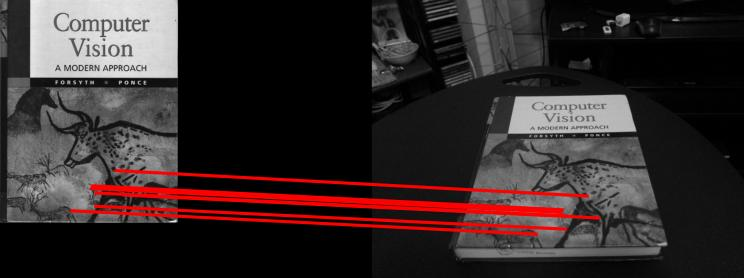
\includegraphics[width=0.75\linewidth]{plotMatches_ratio_0.5_sigma_0.10.jpg} \\
            Figure X plotMatches with ratio = 0.5 and sigma = 0.10 \\~\\
            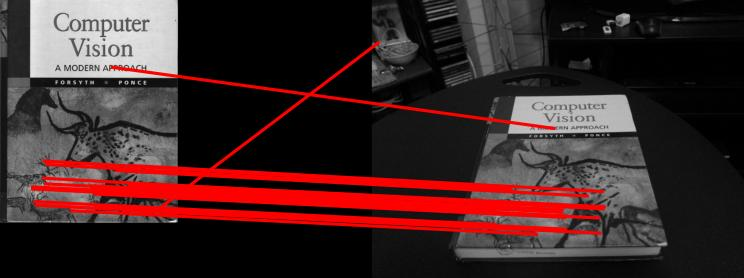
\includegraphics[width=0.75\linewidth]{plotMatches_ratio_0.6_sigma_0.10.jpg} \\
            Figure X plotMatches with ratio = 0.6 and sigma = 0.10 \\~\\
            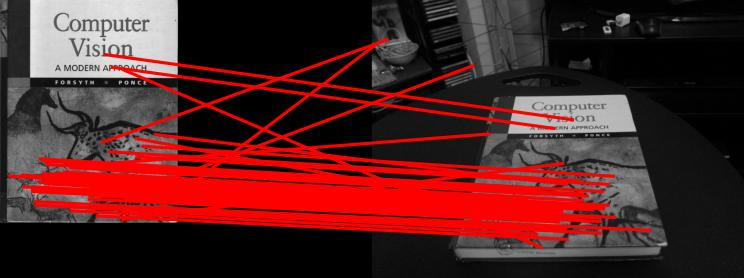
\includegraphics[width=0.75\linewidth]{plotMatches_ratio_0.7_sigma_0.10.jpg} \\
            Figure X plotMatches with ratio = 0.7 and sigma = 0.10 \\~\\
            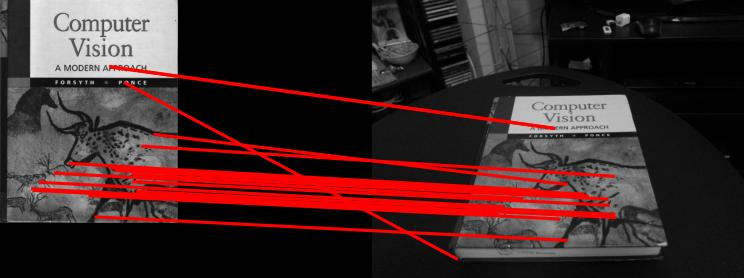
\includegraphics[width=0.75\linewidth]{plotMatches_ratio_0.7_sigma_0.15.jpg} \\
            Figure X plotMatches with ratio = 0.7 and sigma = 0.15 \\~\\
            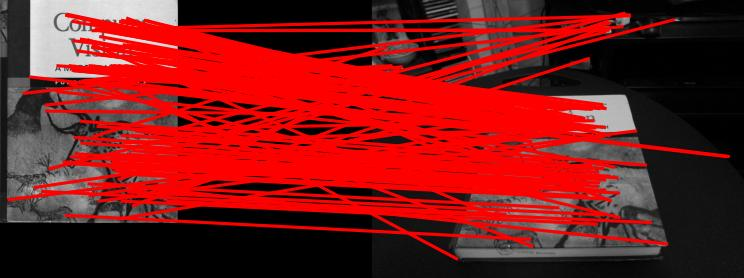
\includegraphics[width=0.75\linewidth]{plotMatches_ratio_1.0_sigma_0.20.jpg} \\
            Figure X plotMatches with ratio = 1.0 and sigma = 0.20 \\~\\
            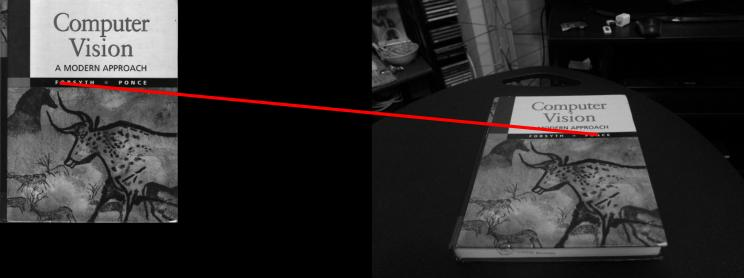
\includegraphics[width=0.75\linewidth]{plotMatches_ratio_1.0_sigma_0.65.jpg} \\
            Figure X plotMatches with ratio = 1.0 and sigma = 0.65
        \end{center}
        We want to have precise matches with the most amount of lines possible. Looks like we'll get it with ratio = 0.5.
        \begin{center}
            \begin{tabular}{|c|c|c|c|}
                \hline
                \textbf{Ratio} & \textbf{Sigma} & \textbf{Matches} & \textbf{Computing time (s)} \\
                \hline
                0.5 & 0.01 & 6 & 170.796 \\
                \hline
                0.5 & 0.02 & 5 & 101.931 \\
                \hline
                0.5 & 0.03 & 8 & 73.038 \\
                \hline
                0.5 & 0.04 & 7 & 45.734 \\
                \hline
                0.5 & 0.05 & 8 & 50.364 \\
                \hline
                0.5 & 0.06 & 7 & 38.476 \\
                \hline
                0.5 & 0.07 & 11 & 30.491 \\
                \hline
                0.5 & 0.08 & 7 & 25.516 \\
                \hline
                0.5 & 0.09 & 7 & 22.290 \\
                \hline
            \end{tabular}
        \end{center}
        Based on the computing time and number of matches, we will choose ratio = 0.5 and sigma = 0.07 as the best parameters.
        \begin{center}
            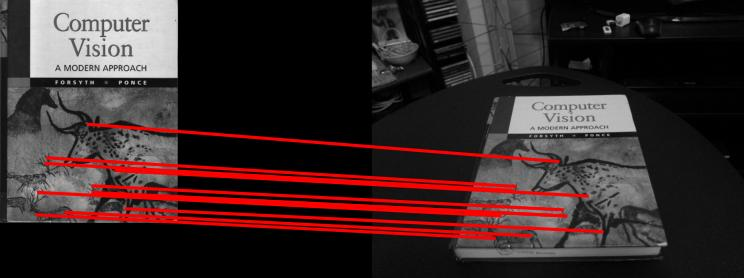
\includegraphics[width=0.75\linewidth]{plotMatches_ratio_0.5_sigma_0.07.jpg}\\
            Figure X plotMatches with best parameters ratio = 0.5 and sigma = 0.07.
        \end{center}

    \end{solution}
    \pagebreak

    \question \textbf{Q2.1.5 BRIEF and Rotations} \\
    Let's investigate how BRIEF works with rotations. Write a script \texttt{briefRotTest.py} that:

    \begin{itemize}
        \item Takes the \texttt{cv\_cover.jpg} and matches it to itself rotated [Hint: use \texttt{scipy.ndimage.rotate}] increments of 10 degrees.
        \item Stores a histogram of the count of matches for each orientation.
        \item Plots the histogram using \texttt{matplotlib.pyplot.hist}
    \end{itemize}

    Visualize the feature matching result at three different orientations and include them in your write-up. Explain why you think the BRIEF descriptor behaves this way.

    \begin{solution}
        \begin{center}
            \centering
            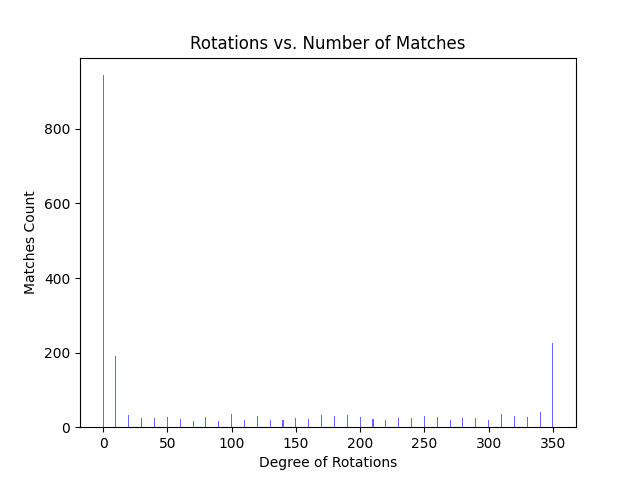
\includegraphics[width=0.75\linewidth]{rotations_plot.png}\\
            Figure X Plot of matches at every 10-degree rotation with sigma = 0.15 and ratio = 0.8.\\~\\
            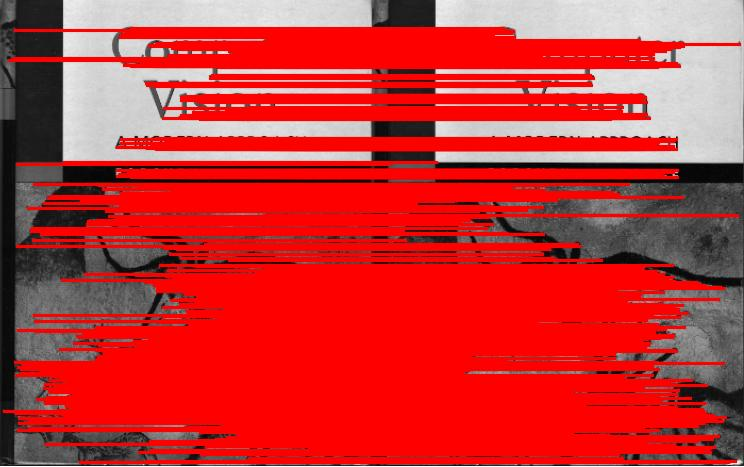
\includegraphics[width=0.6\linewidth]{plotMatches_rotation_0.jpg}\\
            Figure X plotMatches with default parameters at 0 degrees with 945 matches.\\~\\
            \centering
            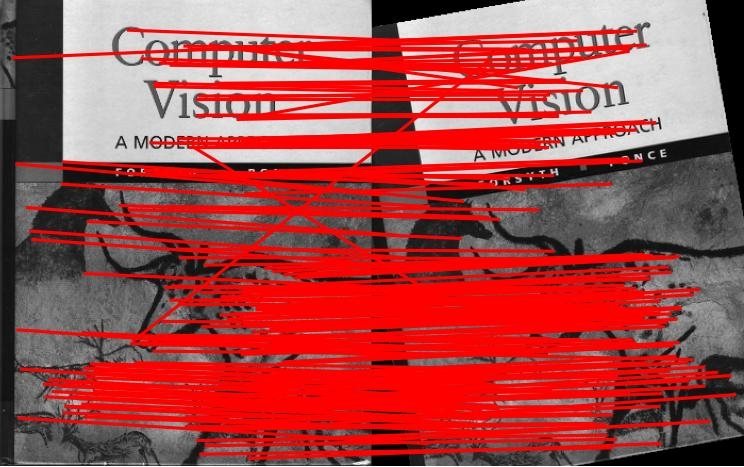
\includegraphics[width=0.6\linewidth]{plotMatches_rotation_10.jpg}\\
            Figure X plotMatches with default parameters at 10 degrees with 195 matches.\\~\\
            \centering
            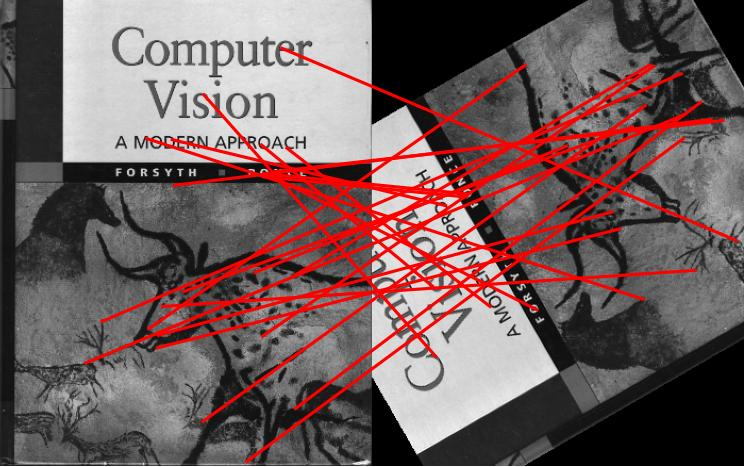
\includegraphics[width=0.6\linewidth]{plotMatches_rotation_120.jpg}\\
            Figure X plotMatches with default parameters at 120 degrees with 24 matches.\\~\\
        \end{center}
        \textbf{Explanation} \\~\\
        BRIEF descriptor works by selecting pixels that are predefined and fixed around a keypoint. Rotation to the images causes these pixels to not correspond to the original keypoint anymore as the binary strings would be different. As its original paper states, the BRIEF descriptor was not designed to be rotationally invariant. However, it still tolerates a few amount of rotations up to 10 degrees. \\~\\
        \textbf{References}
        \begin{enumerate}
            \item https://medium.com/@deepanshut041/introduction-to-brief-binary-robust-independent-elementary-features-436f4a31a0e6
            \item M. Calonder, V. Lepetit, C. Strecha, and P. Fua, "BRIEF: Binary Robust Independent Elementary Features," in Proceedings of the 11th European Conference on Computer Vision (ECCV), 2010.
        \end{enumerate}
    \end{solution}
    

    \pagebreak
    
    \begingroup
    \large \textbf{Homography Computation}
    \endgroup
    
    \question \textbf{Q2.2.1 Computing the Homography}\\
    Write a function \texttt{computeH} that estimates the planar homography from a set of matched point pairs.
    \[
        \texttt{H2to1 = computeH(x1, x2)}
    \]
    \texttt{x1} and \texttt{x2} are $N \times 2$ matrices containing the coordinates $(x, y)$ of point pairs between the two images. \texttt{H2to1} should be a $3 \times 3$ matrix for the best homography from image 2 to image 1 in the least-square sense. The \texttt{numpy.linalg} functions \texttt{eig} or \texttt{svd} will be useful to get the eigenvectors (see Section 1 of this handout for details).

    \begin{solution}
    (Note the indentation that occurs because the line is too long for the solution box so it has to broken down into two lines, even though when it is actually typed and ran in Python, should be typed in one line.)
        \begin{verbatim}
def computeH(x1, x2):
    # Q2.2.1
    # Compute the homography between two sets of points
    
    # INPUTS
    # x1 : N x 2 matrix; coordinates of point pairs between two
        images in image 1
    # x2 : N x 2 matrix; coordinates of point pairs between two
        images in image 2
    
    # OUTPUTS
    # H2to1 : 3 x 3 matrix; best homography from image 2 to 1 in
        the least-square sense
    
    x1 = x1.T
    x2 = x2.T
    
    N = len(x1)
    
    if N < 4:
        raise ValueError('At least 4 points required to compute
            homography.')
    
    A = np.empty([2 * N, 9])
    for i in range(N):
        x1_xi = x1[i, 0] # x coordinate in x1
        x1_yi = x1[i, 1] # y coordinate in x1
        x2_xi = x2[i, 0] # x coordinate in x2
        x2_yi = x2[i, 1] # y coordinate in x2
        A[2*i] = [x2_xi, x2_yi, 1, 0, 0, 0, -x1_xi * x2_xi,
            -x1_xi * x2_yi, -x1_xi]
        A[2*i + 1] = [0, 0, 0, x2_xi, x2_yi, 1, -x1_yi * x2_xi,
            -x1_yi * x2_yi, -x1_yi]
    
    _, _, V_t = np.linalg.svd(A.T @ A)
    smallest_eigenvector = V_t[-1, :]
    H2to1 = smallest_eigenvector.reshape(3,3)
    return H2to1
        \end{verbatim}
    \end{solution}

    \pagebreak

    \begingroup
    \large \textbf{Homography Normalization}
    \endgroup

    \question \textbf{Q2.2.2 Homography with normalization} \\
    Implement the function \texttt{computeH\_norm}

    \begin{center}
        \texttt{H2to1 = computeH\_norm(x1, x2)}
    \end{center}

    This function should normalize the coordinates in \texttt{x1} and \texttt{x2} and call \texttt{computeH(x1, x2)}.

    \begin{solution}
    (Note the indentation that occurs because the line is too long for the solution box so it has to broken down into two lines, even though when it is actually typed and ran in Python, should be typed in one line.)
        \begin{verbatim}
def computeH_norm(x1, x2):
    # Q2.2.2
    # Compute the centroid of the points
 
    # INPUTS
    # x1 : N x 2 matrix; coordinates of point pairs between two
        images in image 1
    # x2 : N x 2 matrix; coordinates of point pairs between two
        images in image 2
	
    # OUTPUTS
    # H2to1 : 3 x 3 matrix; best homography from image 2 to 1 i
        the least-square sense
    
    # Shift so centroid is at the origin (NOTE: Done in similarity
        transform!)
    # Normalize the points so that the largest distance from the
        origin is equal to sqrt(2)
    
    mean_x1_x = np.mean(x1[:,0])
    mean_x1_y = np.mean(x1[:,1])
    mean_x2_x = np.mean(x2[:,0])
    mean_x2_y = np.mean(x2[:,1])
 
    N1 = x1.shape[0]
    N2 = x2.shape[0]
    s_x1 = np.empty((N1))
    s_x2 = np.empty((N2))

    # Get the scaling factor for both x1 and x2
    for i in range(N1):
        s_x1[i] = np.sqrt((x1[i, 0] - mean_x1_x) ** 2 +
            (x1[i, 1] - mean_x1_y) ** 2)
    x1_scale = np.sqrt(2)/np.amax(s_x1)
    
    for i in range(N2):
        s_x2[i] = np.sqrt((x2[i, 0] - mean_x2_x) ** 2 +
            (x1[i, 1] - mean_x1_y) ** 2)
    x2_scale = np.sqrt(2)/np.amax(s_x2)
    
    # Similarity transform 1: scale and shift (translate)
        the origin
    T1 = np.array([
        [x1_scale, 0, -x1_scale * mean_x1_x],
        [0, x1_scale, -x1_scale * mean_x1_y],
        [0, 0, 1]
    ])
 
    x1_normalized = np.hstack((x1, np.ones((N1, 1))))
    x1_hom = T1 @ x1_normalized.T
    
    # Similarity transform 2
    T2 = np.array([
        [x2_scale, 0, -x2_scale * mean_x2_x],
        [0, x2_scale, -x2_scale * mean_x2_y],
        [0, 0, 1]
    ])
    x2_normalized = np.hstack((x2, np.ones((N2, 1))))
    x2_hom = T2 @ x2_normalized.T
 
    # Compute homography
    H2to1_normalized = computeH(x1_hom, x2_hom)
    
    # Denormalization
    H2to1 = np.linalg.inv(T2) @ H2to1_normalized @ T1
    return H2to1
        \end{verbatim}
    \end{solution}

    \pagebreak

    \begingroup
    \large \textbf{RANSAC}
    \endgroup

    \question \textbf{Q2.2.3 Implement RANSAC for computing a homography} \\

    Write a function:
    \begin{center}
        \texttt{bestH2to1, inliers = computeH\_ransac(locs1, locs2)}
    \end{center}

    where \texttt{bestH2to1} should be the homography \(\mathbf{H}\) with most inliners found during RANSAC. \(\mathbf{H}\) will be a homography such that if \(\mathbf{x_2}\) is a point in \texttt{locs2} and \(\mathbf{x_1}\) is a corresponding point in \texttt{locs1}, then \(\mathbf{x_1} \equiv \mathbf{Hx_2}\). \texttt{locs1} and \texttt{locs2} are $N \times 2$ matrices containing the matched points. \texttt{inliers} is a vector of length $N$ with a 1 at those matches that are part of the consensus set, and 0 elsewhere. Use \texttt{computeH\_norm} to compute the homography.

    \begin{solution}
        (Note the indentation that occurs because the line is too long for the solution box so it has to broken down into two lines, even though when it is actually typed and ran in Python, should be typed in one line.)
        \begin{verbatim}
def computeH_ransac(locs1, locs2, iters=700, thres=2.0):
    # Q2.2.3
    # Compute the best fitting homography given a list of matching
        points
    
    # INPUTS
    # locs1 : N x 2 matrix, each row has (x, y) of a feature point
    # locs2 : N x 2 matrix, each row has (x, y) of a feature point
    # iters : max number of iterations
    # thres : threshold to determine inliers
    
    # OUTPUTS
    # bestH2to1 : best homography designated by ransac algorithm
    # inliers : vector of length N with a 1 at matches
    
    N = len(locs1)
    inliers = np.zeros((1, N))
    bestH2to1 = np.zeros((3,3))
    
    for i in range(iters):
        # pick 4 random points
        idx = np.random.choice(N, size=4, replace=False)
        x1 = locs1[idx]
        x2 = locs2[idx]

        # compute homography
        H2to1 = computeH_norm(x1, x2)
        temp_inliers = np.zeros((N, 1))
    
        # transform the points so we can see where points in locs2
            would appear in locs1
        for j in range(N):
            # convert locs1 point to homogeneous coordinates
            x1_homogenous = np.hstack((locs1[j] , 1))
    
            # apply homography transformation
            x2_calc = np.dot(H2to1, x1_homogenous)
            x2_calc = x2_calc / x2_calc[2] # normalize to make
                homogenous
            x2_calc = x2_calc[:2]
    
            # calculate euclidean distance between projection and
                original point in locs2
            l2_dist = np.linalg.norm(locs2[j] - x2_calc)
    
            if l2_dist < thres:
                temp_inliers[j] = 1
    
        if np.sum(temp_inliers) > np.sum(inliers):
            inliers = temp_inliers.T
            bestH2to1 = H2to1
    
    return bestH2to1, inliers
        \end{verbatim}
    \end{solution}

    \pagebreak

    \begingroup
    \large \textbf{Automated Homography Estimation and Warping}
    \endgroup

    \question \textbf{Q2.2.4 Putting it together} \\
    Write a script \texttt{HarryPoterize.py} that
    \begin{enumerate}
        \item Reads \texttt{cv\_cover.jpg}, \texttt{cv\_desk.png}, and \texttt{hp\_cover.jpg}.
        \item Computes a homography automatically using \texttt{MatchPics} and \texttt{computeH\_ransac}.
        \item Uses the computed homography to wrap \texttt{hp\_cover.jpg} to the dimension of the \texttt{cv\_desk.png} image using the \texttt{skimage} function \texttt{skimage.transform.warp} or OpenCV function \texttt{cv2.warpPerspective}.
        \item At this point you should notice that although the image is being warped to the correct location, it is not filling up the same space as the book. Why do you think this is happening? How would you modify \texttt{hp\_cover.jpg} to fix this issue?
        \item Implement the function:
            \begin{center}
                \texttt{composite\_img} = \texttt{compositeH(H2to1, template, img)}
            \end{center}
            to now compose this warped image with the desk image.
        \item Include your result in the write-up.
    \end{enumerate}

    \begin{solution}
    Having experimented and assuming that the best parameters have been derived from \textbf{Q2.1.4}, we assume that the best parameters to start with is ratio = 0.5 and sigma = 0.07. We first experiment with the number of the maximum iterations for the RANSAC algorithm, \texttt{iters}, and threshold for a data to be count as an inlier, \texttt{thres}.
    \begin{center}
        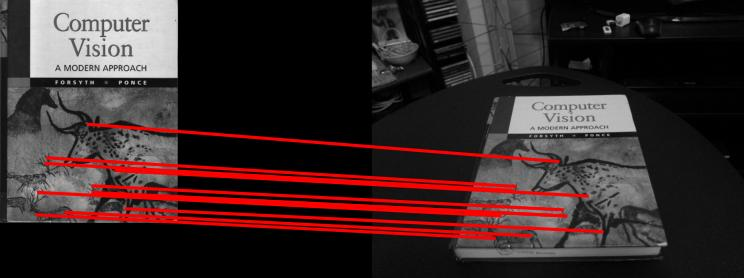
\includegraphics[width=0.75\linewidth]{plotMatches_ratio_0.5_sigma_0.07.jpg}\\
        Figure X plotted matches at ratio = 0.5 and sigma = 0.07\\~\\
        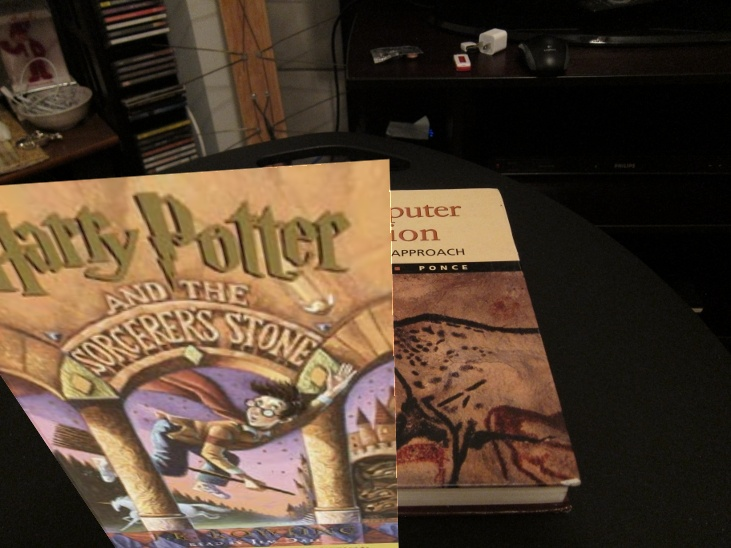
\includegraphics[width=0.4\linewidth]{desk_r0.5_s0.07_i2000_t50.jpg}\\
        Figure X HarryPotterize'd textbook on desk \\ with \texttt{iters} = 2000 and \texttt{thres} = 50. \\~\\
        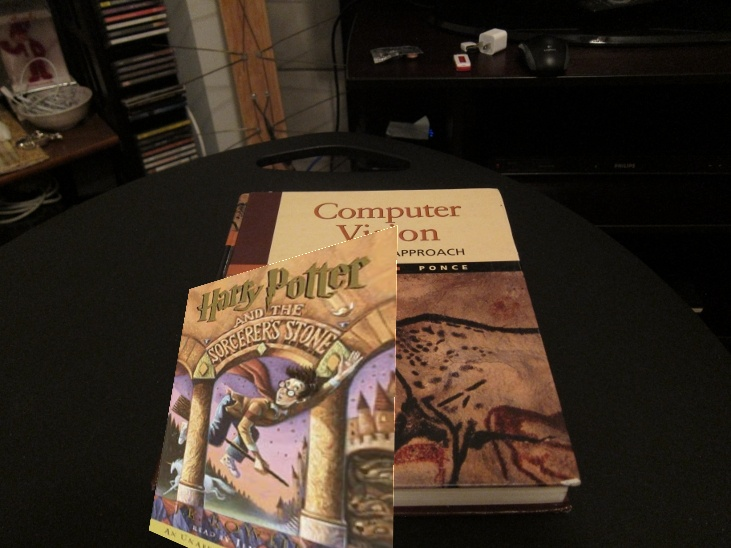
\includegraphics[width=0.4\linewidth]{desk_r0.5_s0.07_i2000_t30.jpg}\\
        Figure X HarryPotterize'd textbook on desk \\ with \texttt{iters} = 2000 and \texttt{thres} = 30. \\~\\
        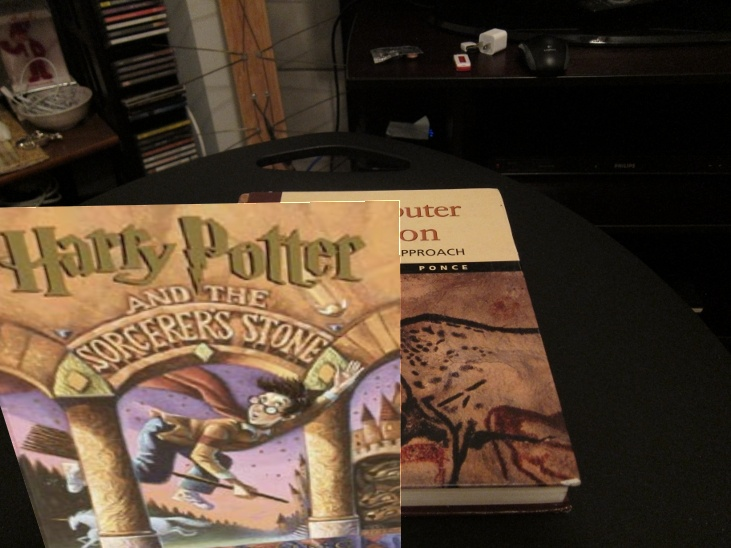
\includegraphics[width=0.4\linewidth]{desk_r0.5_s0.07_i2000_t10.jpg}\\
        Figure X HarryPotterize'd textbook on desk \\ with \texttt{iters} = 2000 and \texttt{thres} = 10.
    \end{center}
    Experimenting with the threshold yielded no good results. The size from \texttt{thres} = 50 and 10 seemed quite correct, but it isn't as positioned well as the one in \texttt{thres} = 30. We'll try lowering the maximum iterations.
    \begin{center}
        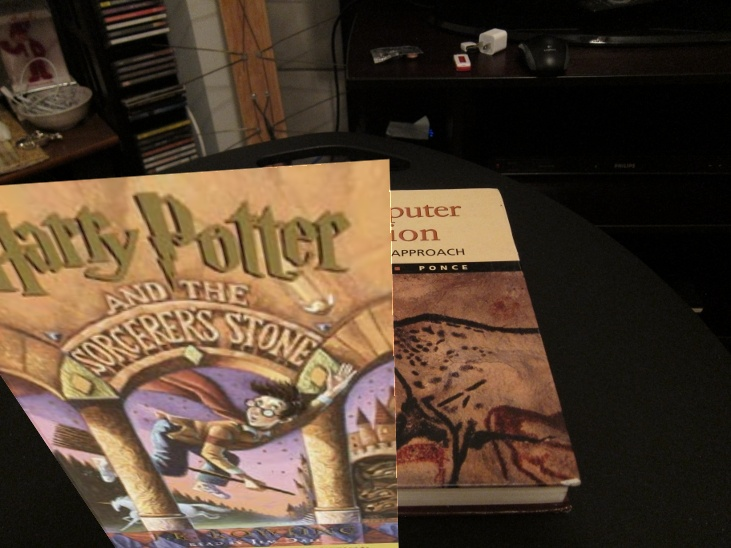
\includegraphics[width=0.4\linewidth]{desk_r0.5_s0.07_i1000_t50.jpg}\\
        Figure X HarryPotterize'd textbook on desk \\ with \texttt{iters} = 1000 and \texttt{thres} = 50. \\-\\
        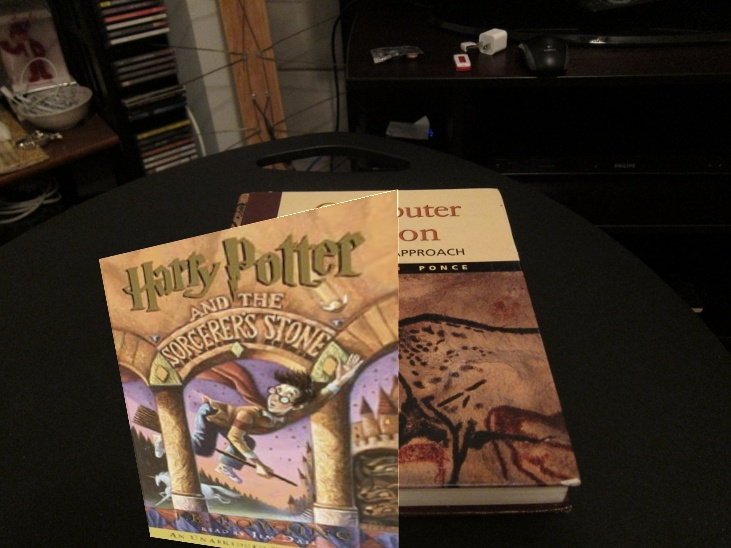
\includegraphics[width=0.4\linewidth]{desk_r0.5_s0.07_i1000_t30.jpg}\\
        Figure X HarryPotterize'd textbook on desk \\ with \texttt{iters} = 1000 and \texttt{thres} = 30. \\-\\
        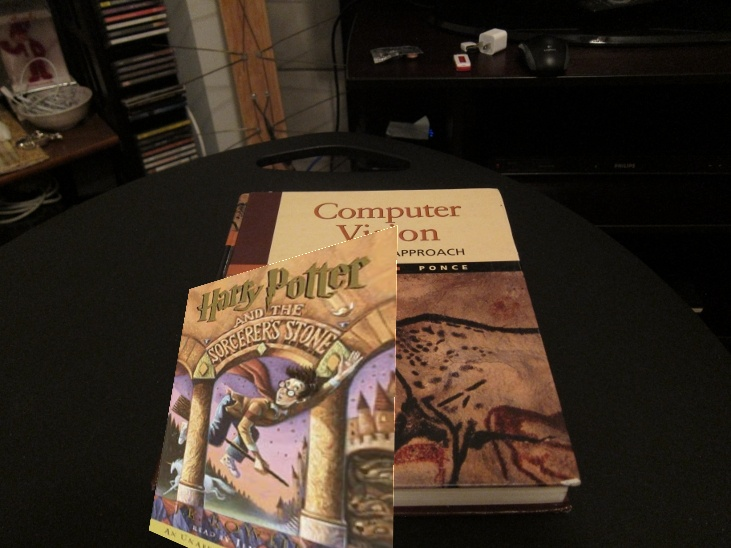
\includegraphics[width=0.4\linewidth]{desk_r0.5_s0.07_i700_t30.jpg}\\
        Figure X HarryPotterize'd textbook on desk \\ with \texttt{iters} = 700 and \texttt{thres} = 30. \\
    \end{center}
    Unfortunately, they weren't good enough either. Varying the ratio and sigma didn't result in a perfect projection either.\\
    \begin{center}
        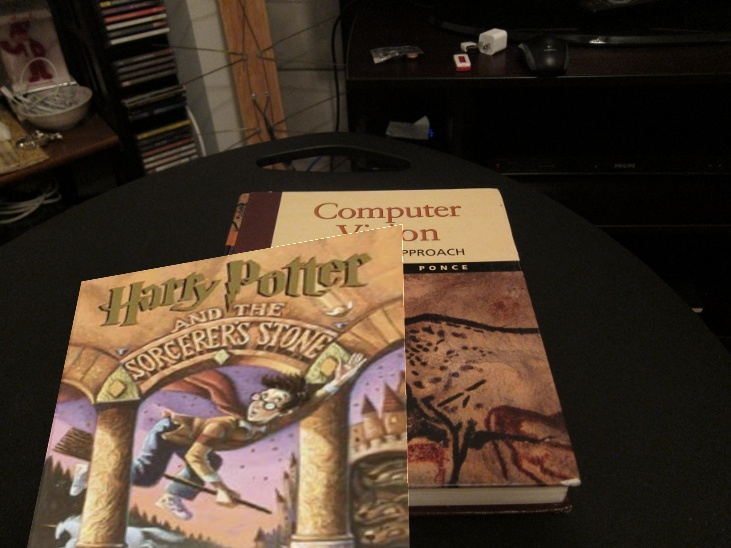
\includegraphics[width=0.4\linewidth]{desk_r0.6_s0.15_i1000_t50.jpg}\\
        Figure X HarryPotterize'd textbook on desk \\ with \texttt{iters} = 1000, \texttt{thres} = 50, \texttt{ratio} = 0.6, \texttt{sigma} = 0.15.
    \end{center}
    \textbf{It should be noted, however, that most projections happened with a better accuracy when done with \texttt{iters} = 1000 and \texttt{thres} = 30.} \\~\\
    \begingroup
        \Large \textbf{Why it isn't perfect}
    \endgroup
        \begin{enumerate}
            \item \textbf{Imperfect matching/Lack of matches}. When doing experiments with the pictures, I had found it interesting that most matches were spread out on the right side of the book cover in \texttt{cv\_desk.png}, while being spread out on the left side of \texttt{cv\_cover.jpg}. There are also instances where parts of \texttt{cv\_cover.jpg} were being matched with other objects in \texttt{cv\_desk.png}. These lack of matches and imperfect matching could be the reason why \texttt{HarryPotterize.py} projections aren't perfect.
            \item \textbf{Incorrect parameters}. It is undeniable that with more and more experimets, the right parameters could be chosen. Alas, it couldn't be found for now.
        \end{enumerate}
    \end{solution}

    \pagebreak

    \begingroup
    \large \textbf{Creating your Augmented Reality Application}
    \endgroup

    \question \textbf{Q3.1 Incorporating video}\\
    Now with the code you have, you're able to create your own Augmented Reality application. What you're going to do is \texttt{HarryPoterize} the video \texttt{ar\_source.mov} onto the \texttt{book.mov}. More specifically, you're going to track the computer vision text book in each frame of \texttt{ar\_source.mov} onto the book in \texttt{book.mov}. Please write a script \texttt{ar.m} to implement this AR application and save your rest video as \texttt{ar.avi} in the \texttt{result/} directory. You may use the function \texttt{loadVid} that we provide to load the videos. Your result should be similar to the LifePrint project. \\
    Note that the book and the videos we have provided have very different aspect ratios (the ratio of the image width to the image height). You must crop each frame to fit onto the book cover. You should crop each frame such that only its central region is used in the final output. \\
    Also, the video \texttt{book.mov} only has translation of objects. If you want to account for rotation of objects, scaling, etc, you would have to pick a better feature point representation (like ORB).

    \begin{solution}
        Blablabla.
    \end{solution}

    \pagebreak 
    \begingroup
    \large \textbf{Extra Credit}
    \endgroup

    \question \textbf{Panorama}

    \begin{solution}
        \begin{center}
            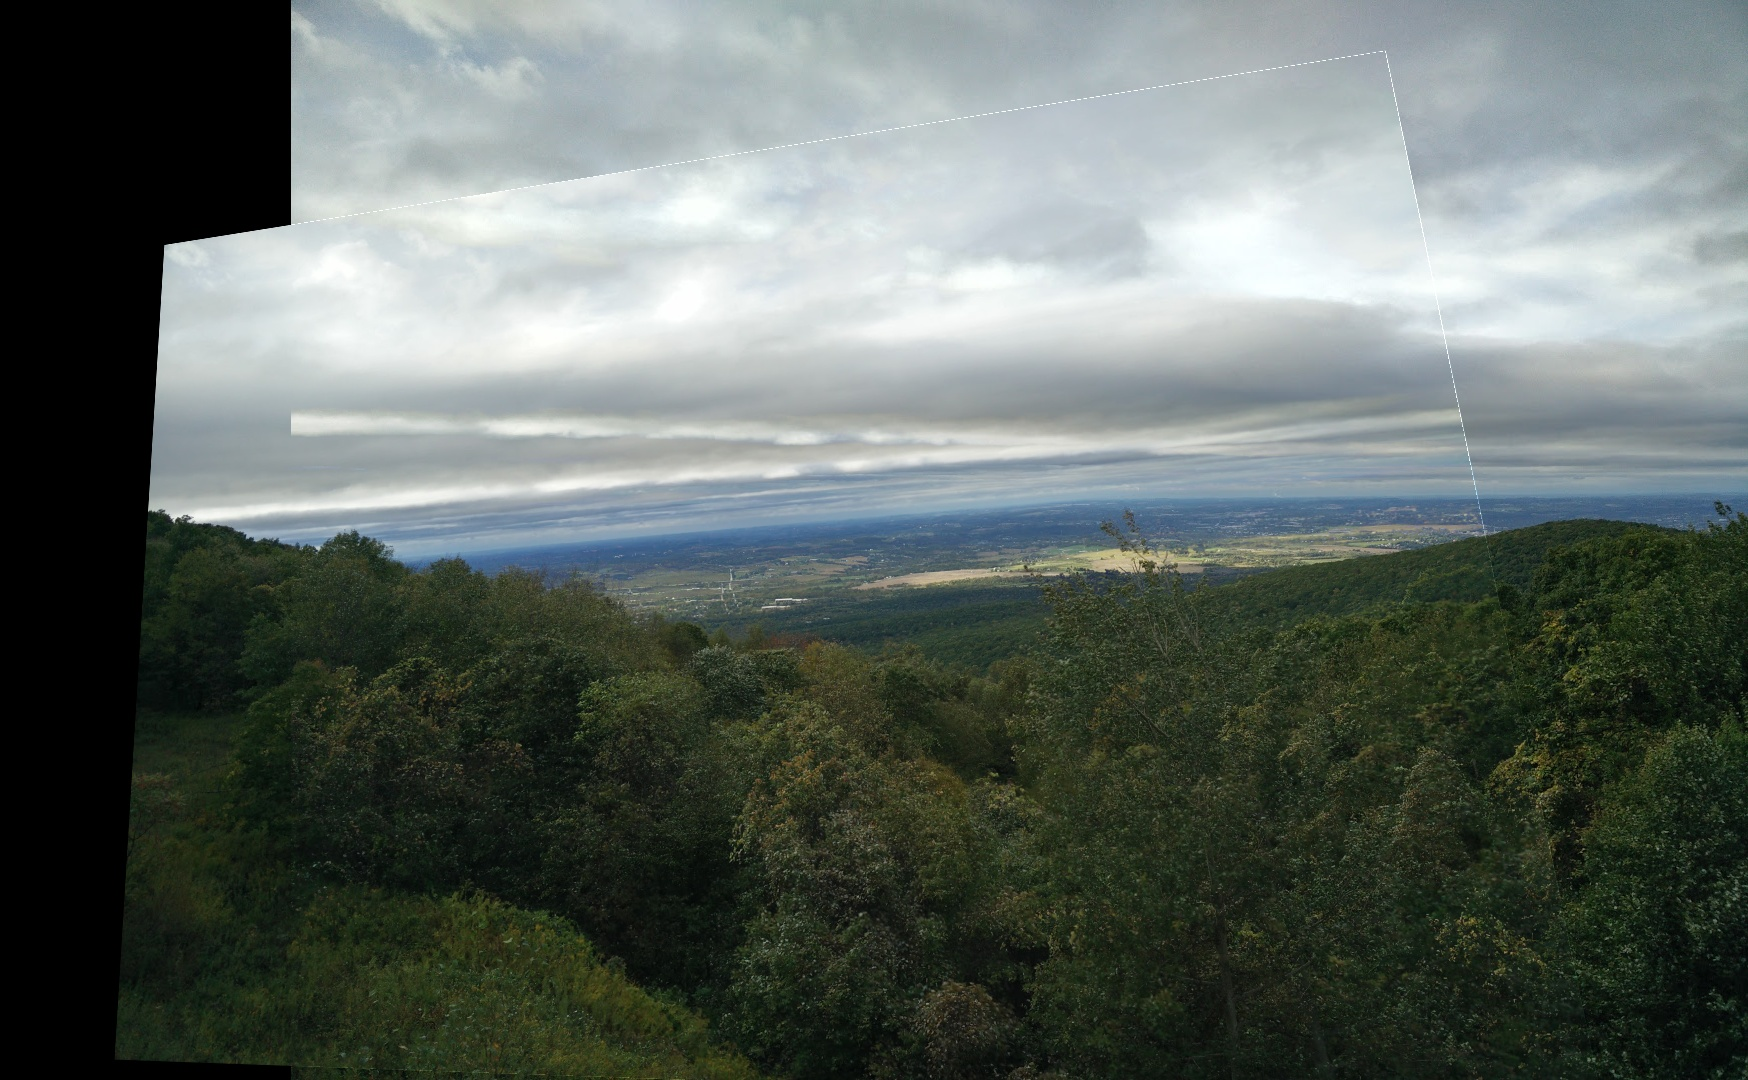
\includegraphics[width=0.5\linewidth]{panorama_stitched_ass.jpg} \\
            Figure X Stitched panorama
        \end{center}
    \end{solution}

    \pagebreak 
    \begingroup
    \large \textbf{Appendix A. Other Experiments}\\
    \endgroup

    \begin{tabular}{|c|c|c|c|}
        \hline
        \textbf{Ratio} & \textbf{Sigma} & \textbf{Matches} & \textbf{Computing time (s)} \\
        \hline
        0.51 & 0.03 & 10 & 58.804 \\
        \hline
        0.51 & 0.04 & 8 & 53.818 \\
        \hline
        0.51 & 0.05 & 9 & 50.697 \\
        \hline
        0.51 & 0.06 & 8 & 36.605 \\
        \hline
        0.51 & 0.07 & 13 & 32.968 \\
        \hline
        0.51 & 0.08 & 9 & 25.079 \\
        \hline
        0.51 & 0.09 & 9 & 19.862 \\
        \hline
        0.52 & 0.03 & 13 & 84.578 \\
        \hline
        0.52 & 0.04 & 11 & 59.944 \\
        \hline
        0.52 & 0.05 & 12 & 39.064 \\
        \hline
        0.52 & 0.06 & 10 & 27.844 \\
        \hline
        0.52 & 0.07 & 15 & 23.871 \\
        \hline
        0.52 & 0.08 & 14 & 24.793 \\
        \hline
        0.52 & 0.09 & 12 & 17.267 \\
        \hline
        0.53 & 0.03 & 16 & 80.189 \\
        \hline
        0.53 & 0.04 & 12 & 57.234 \\
        \hline
        0.53 & 0.05 & 13 & 49.668 \\
        \hline
        0.53 & 0.06 & 11 & 35.337 \\
        \hline
        0.53 & 0.07 & 16 & 26.040 \\
        \hline
        0.53 & 0.08 & 14 & 20.795 \\
        \hline
        0.53 & 0.09 & 12 & 18.618 \\
        \hline
        0.54 & 0.03 & 18 & 66.883 \\
        \hline
        0.54 & 0.04 & 16 & 44.481 \\
        \hline
        0.54 & 0.05 & 16 & 37.272 \\
        \hline
        0.54 & 0.06 & 15 & 35.396 \\
        \hline
        0.54 & 0.07 & 19 & 27.611 \\
        \hline
        0.54 & 0.08 & 14 & 22.775 \\
        \hline
        0.54 & 0.09 & 13 & 21.168 \\
        \hline
    \end{tabular}
    
\end{questions}
\end{document}